%%
%%  Annexes
%%
%%  Note: Ne pas modifier la ligne ci-dessous. / Do not modify the following line.
\ifthenelse{\equal{\Langue}{english}}{
	\addcontentsline{toc}{compteur}{APPENDICES}
}{
	\addcontentsline{toc}{compteur}{ANNEXES}
}
%%
%%
%%  Toutes les annexes doivent être inclues dans ce document
%%  les unes à la suite des autres.
%%  All annexes must be included in this document one after the other.
\Annexe{DORA-Explorer: Execution loop}
\label{annexe: execution_loop}

\begin{algorithm}[htbp]
\small
\SetAlgoLined
\DontPrintSemicolon
 $\bm{x} \leftarrow random\_coordinates$\;
 \While{True}{
  $\nabla_r, \nabla_e \longleftarrow (0, 0), (0, 0)$\;
  \;
  \For{$n \in \nu$}{
    $\nabla_r \leftarrow \nabla_r + (r\_stig[\bm{x}] - r\_stig[\bm{n}]) \cdot normalize(\bm{n})$\;
    $\nabla_e \leftarrow \nabla_e + (e\_stig[\bm{x}] - e\_stig[\bm{n}]) \cdot normalize(\bm{n})$\;
  }
  \;
  $\bm{m} \leftarrow \alpha \cdot \nabla_r + \beta \cdot \nabla_e + \gamma \cdot compute\_avoidance(sensors)$\;
  $\bm{x} \leftarrow \bm{x} + k \cdot normalize(\bm{m})$\;
  $r\_stig[\bm{x}], e\_stig[\bm{x}] \leftarrow get\_radiation(), time()$\;
 }
 \caption{DORA Execution Loop}
 \label{alg:dora}
\end{algorithm}


\Annexe{DORA-Explorer: Risk-aware exploration}
\label{annexe: intuition}
\begin{figure*}[htbp]
    \centering
    \subfigure[]
         {
         \centering
         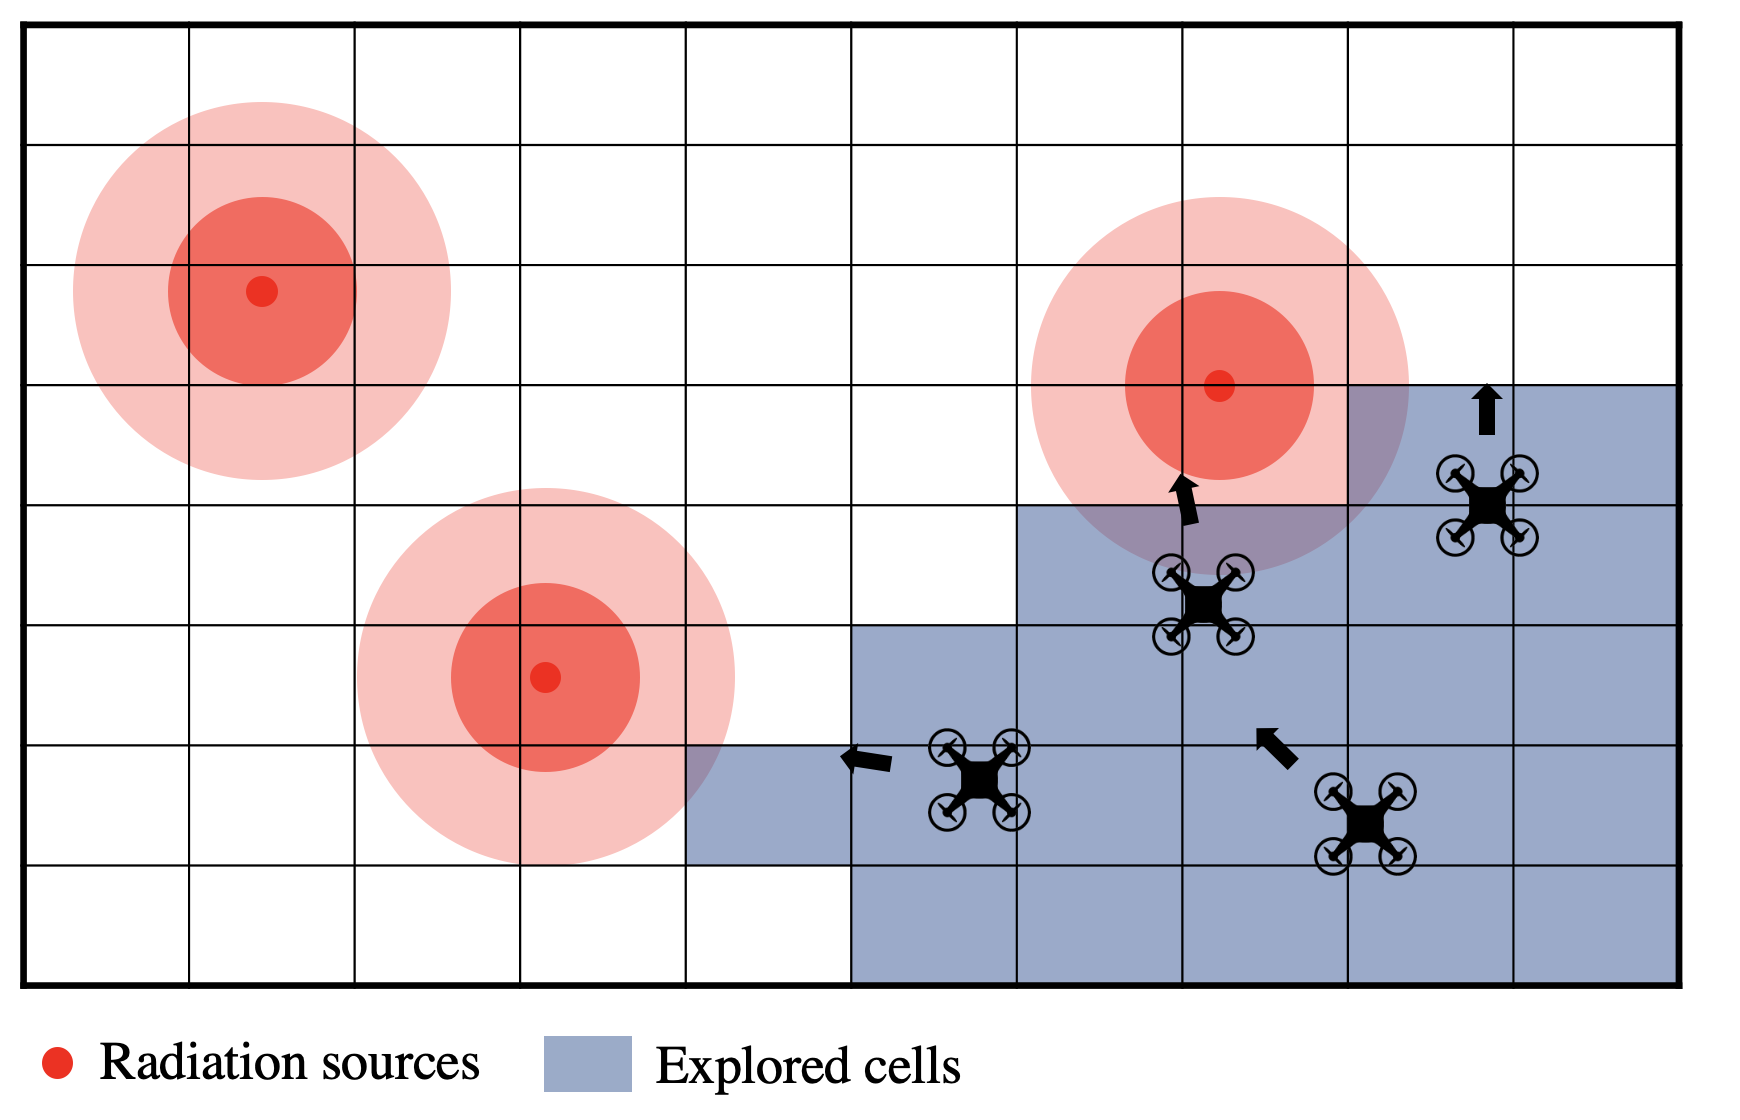
\includegraphics[width=0.47\textwidth]{images/risk_aware_b.png}
         \label{risk_aware_b}
         }
    \hfill
    \subfigure[]
    {
         \centering
         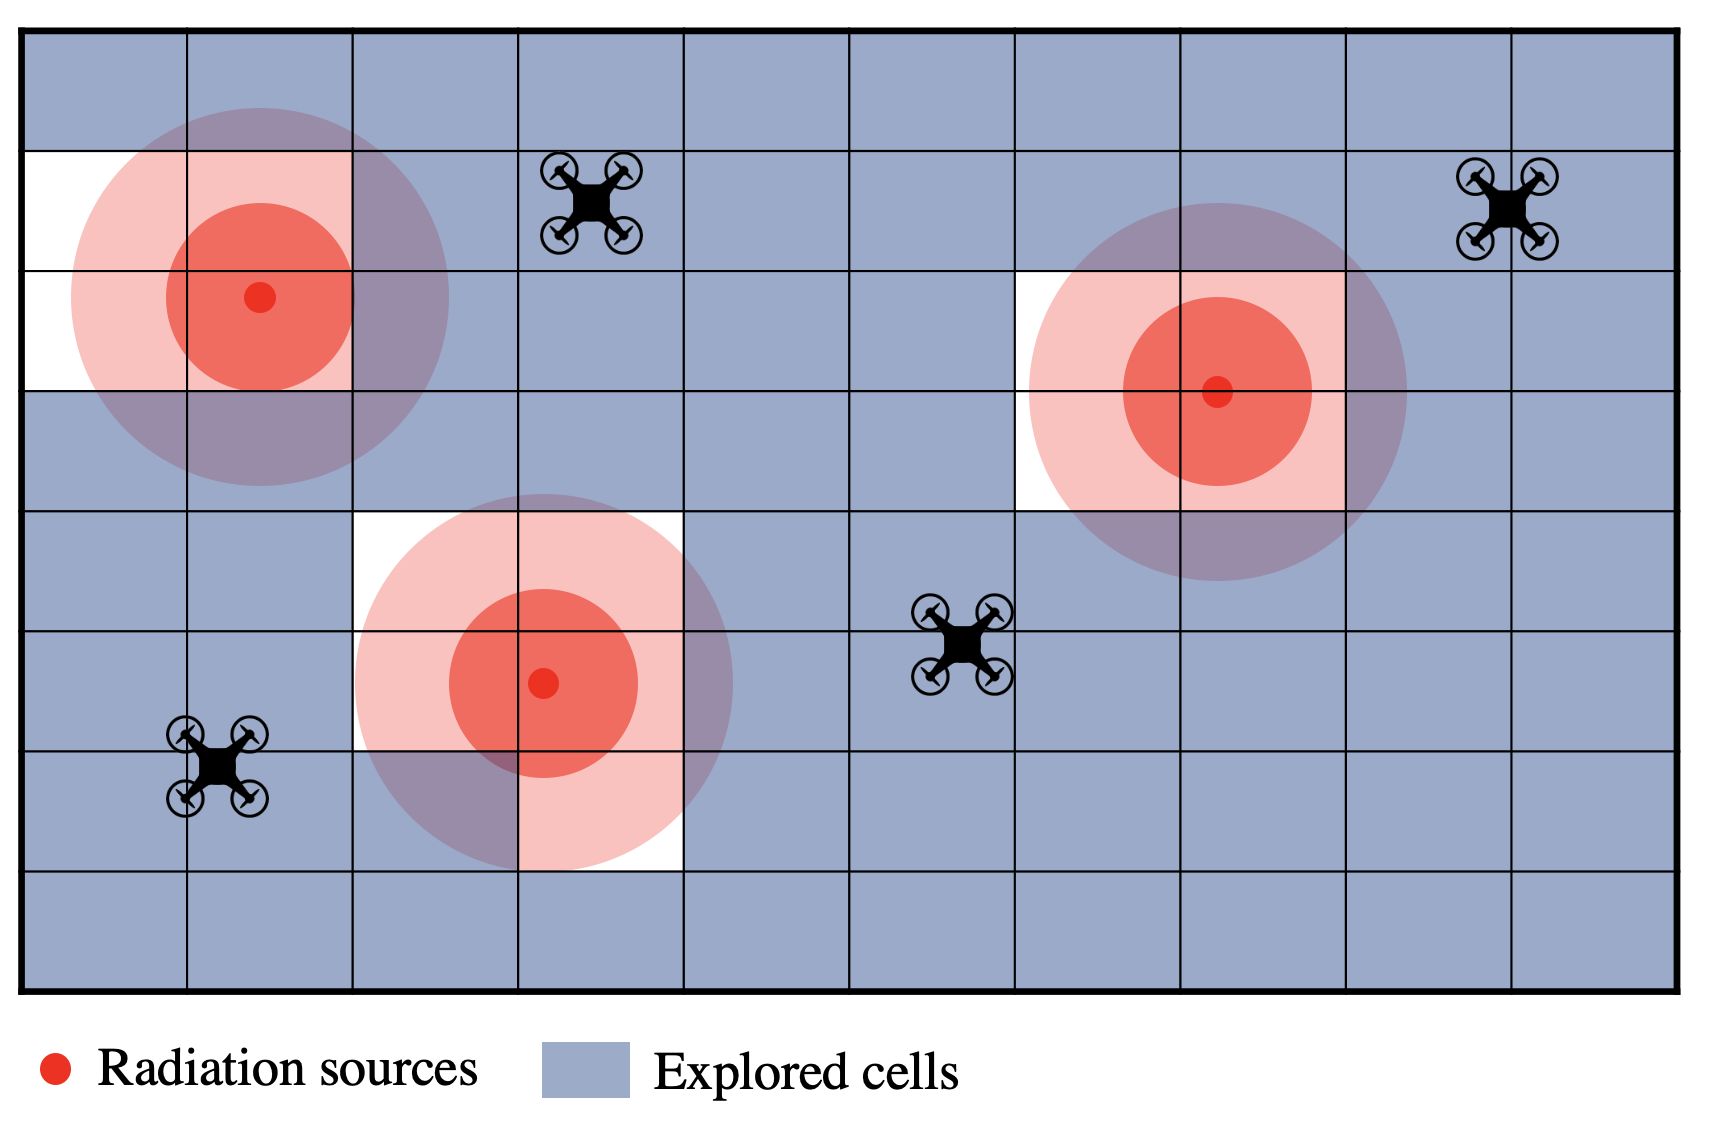
\includegraphics[width=0.47\textwidth]{images/risk_aware_c.png}
         \label{risk_aware_c}
         }
    \hfill
    \subfigure[]{
         \centering
         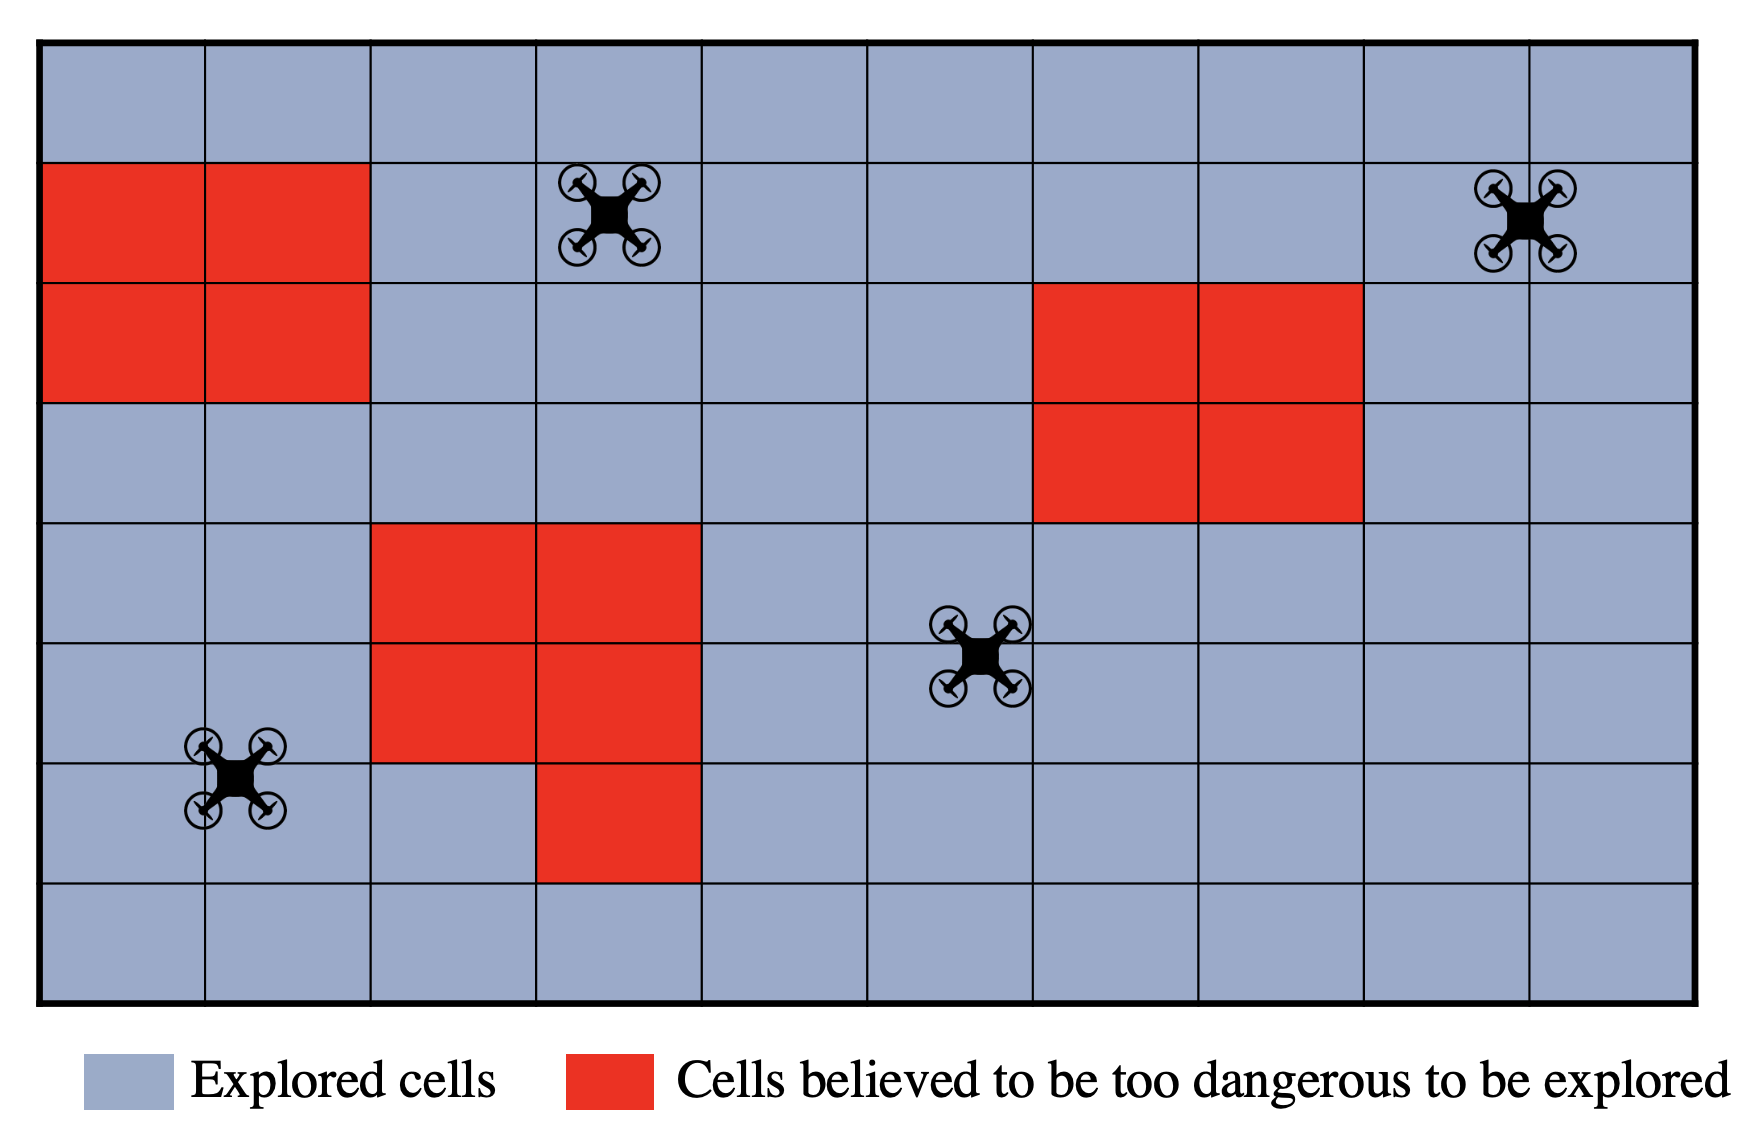
\includegraphics[width=0.47\textwidth]{images/risk_aware_d.png}
         \label{risk_aware_d}}
        \caption{Risk aware exploration intuition. Fig. \ref{risk_aware_b}: Robots start exploring a hazardous environment. When a new cell is explored, the sensed radiation is used to update the DBM. Fig. \ref{risk_aware_c}: The cells have been mostly covered by the robots. Fig. \ref{risk_aware_d}: Only cells believed to be too dangerous remain unexplored.}
    \label{risk_aware}
\end{figure*}

\Annexe{DORA-Explorer: ARGoS simulated environment}
\label{annexe: argos}

\begin{figure}[htbp]
	\centering
    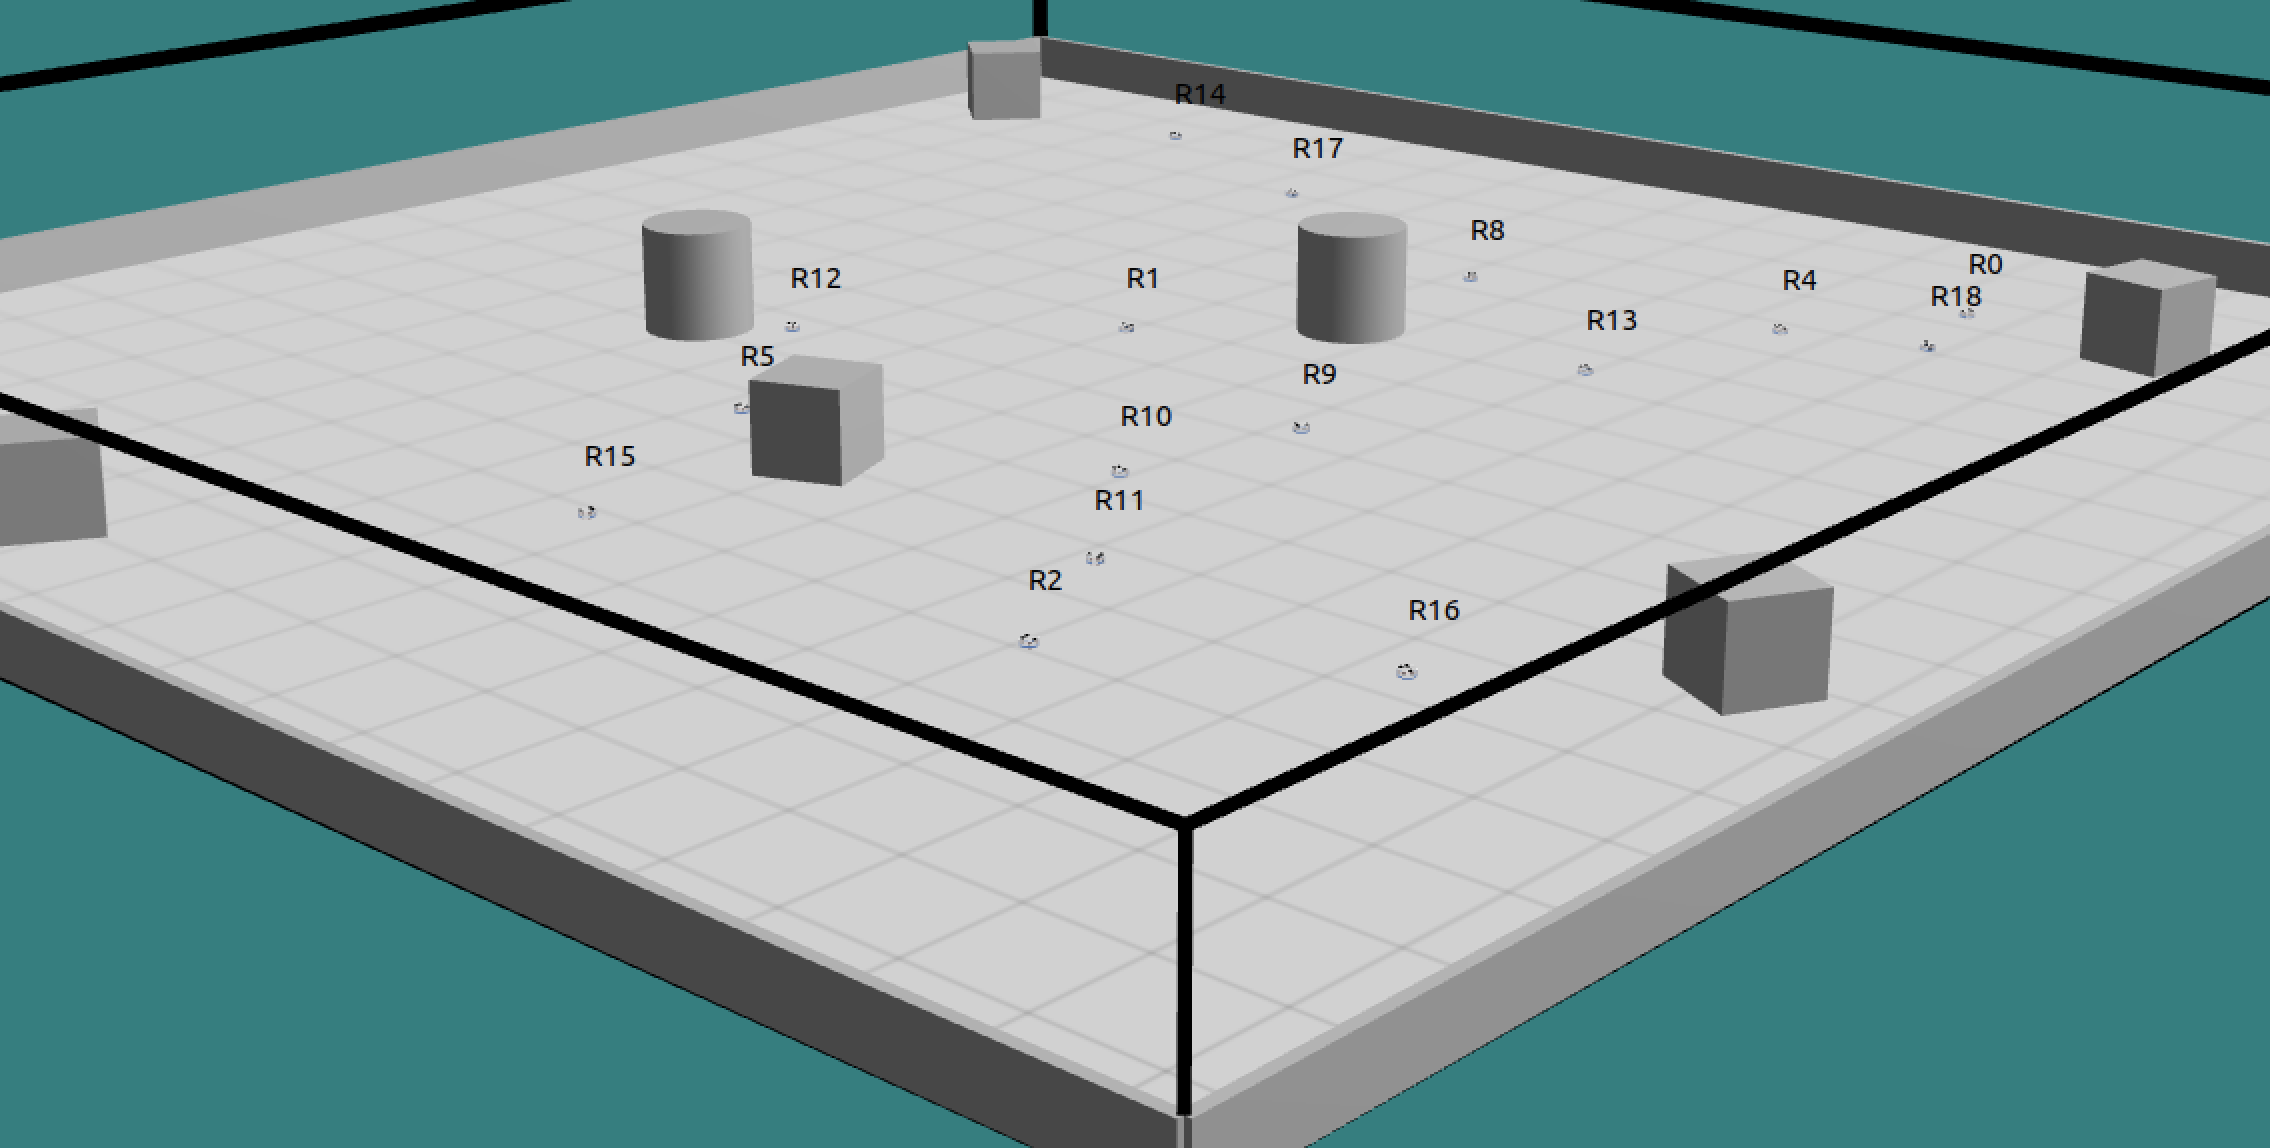
\includegraphics[width=\columnwidth]{images/argos.png}
    \caption{$400 \text{m}^2$ environment in the ARGoS simulator with 20 KheperaIV robots. Cylinders are radiation sources and boxes are random obstacles.}
    \label{argos}
\end{figure}

\Annexe{DORA-Explorer: Results over time}
\label{annexe: results}

\begin{figure}[htbp]
	\centering
    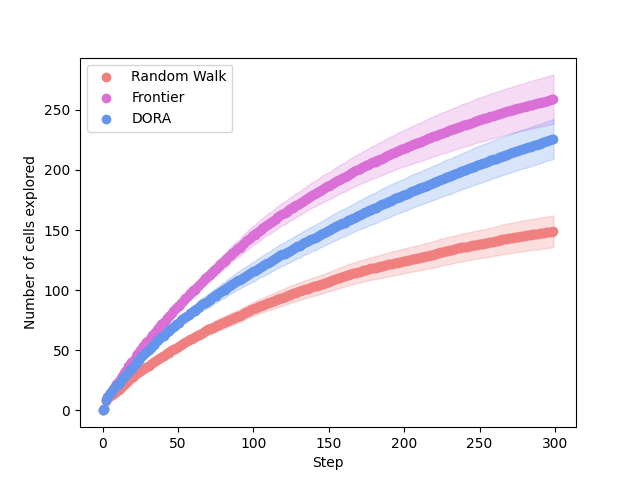
\includegraphics[width=0.53\columnwidth]{images/explored_10.png}
    \caption{Performance comparison of DORA, FBE and random walk for number of explored cells over time, with N=10 robots.}
    \label{results:explored10}
\end{figure}

\begin{figure}[htbp]
	\centering
    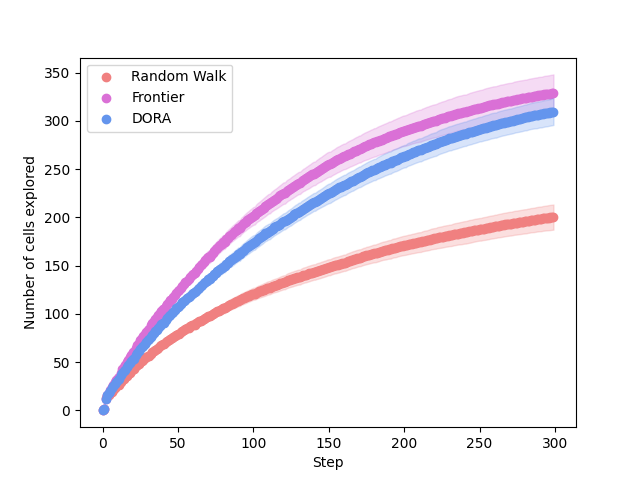
\includegraphics[width=0.53\columnwidth]{images/explored_15.png}
    \caption{Performance comparison of DORA, FBE and random walk for number of explored cells over time, with N=15 robots.}
    \label{results:explored15}
\end{figure}

\begin{figure}[htbp]
	\centering
    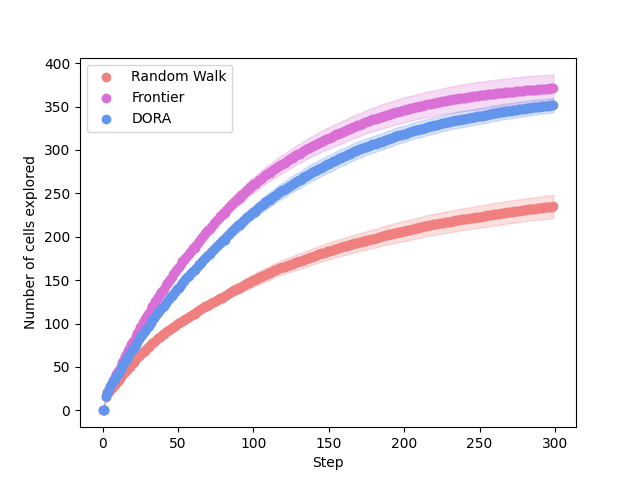
\includegraphics[width=0.53\columnwidth]{images/explored_20.png}
    \caption{Performance comparison of DORA, FBE and random walk for number of explored cells over time, with N=20 robots.}
    \label{results:explored20}
\end{figure}

\begin{figure}[htbp]
	\centering
    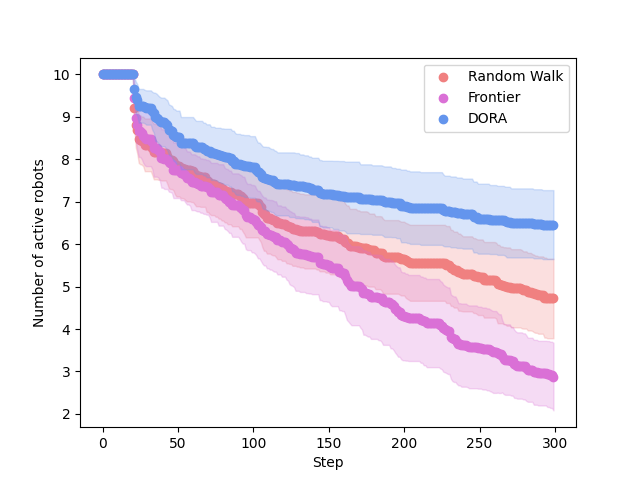
\includegraphics[width=0.53\columnwidth]{images/activerobots_10.png}
    \caption{Performance comparison of DORA, FBE and random walk for number of active robots over time, with N=10 robots.}
    \label{results:failures10}
\end{figure}

\begin{figure}[htbp]
	\centering
    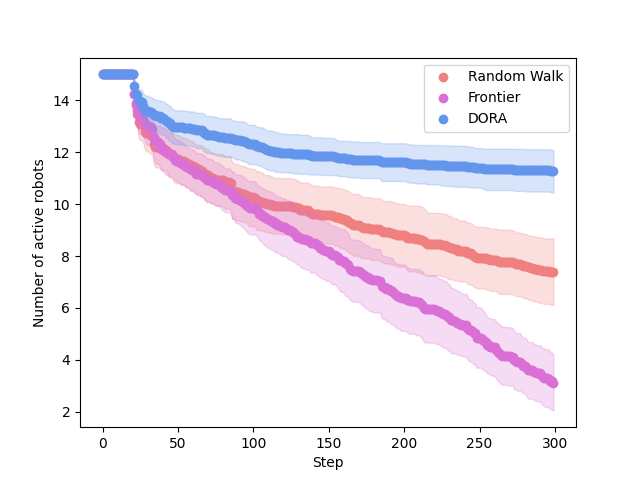
\includegraphics[width=0.53\columnwidth]{images/activerobots_15.png}
    \caption{Performance comparison of DORA, FBE and random walk for number of active robots over time, with N=15 robots.}
    \label{results:failures15}
\end{figure}

\begin{figure}[htbp]
	\centering
    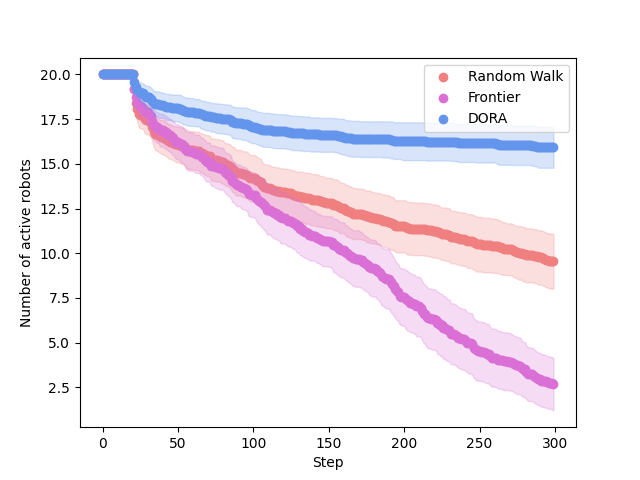
\includegraphics[width=0.53\columnwidth]{images/activerobots_20.png}
    \caption{Performance comparison of DORA, FBE and random walk for number of active robots over time, with N=20 robots.}
    \label{results:failures20}
\end{figure}

\Annexe{DORA-Explorer: Physical experiments}
\label{annexe: physical}
\begin{figure}[htbp]
    \centering
    \captionsetup{belowskip=-20pt}
    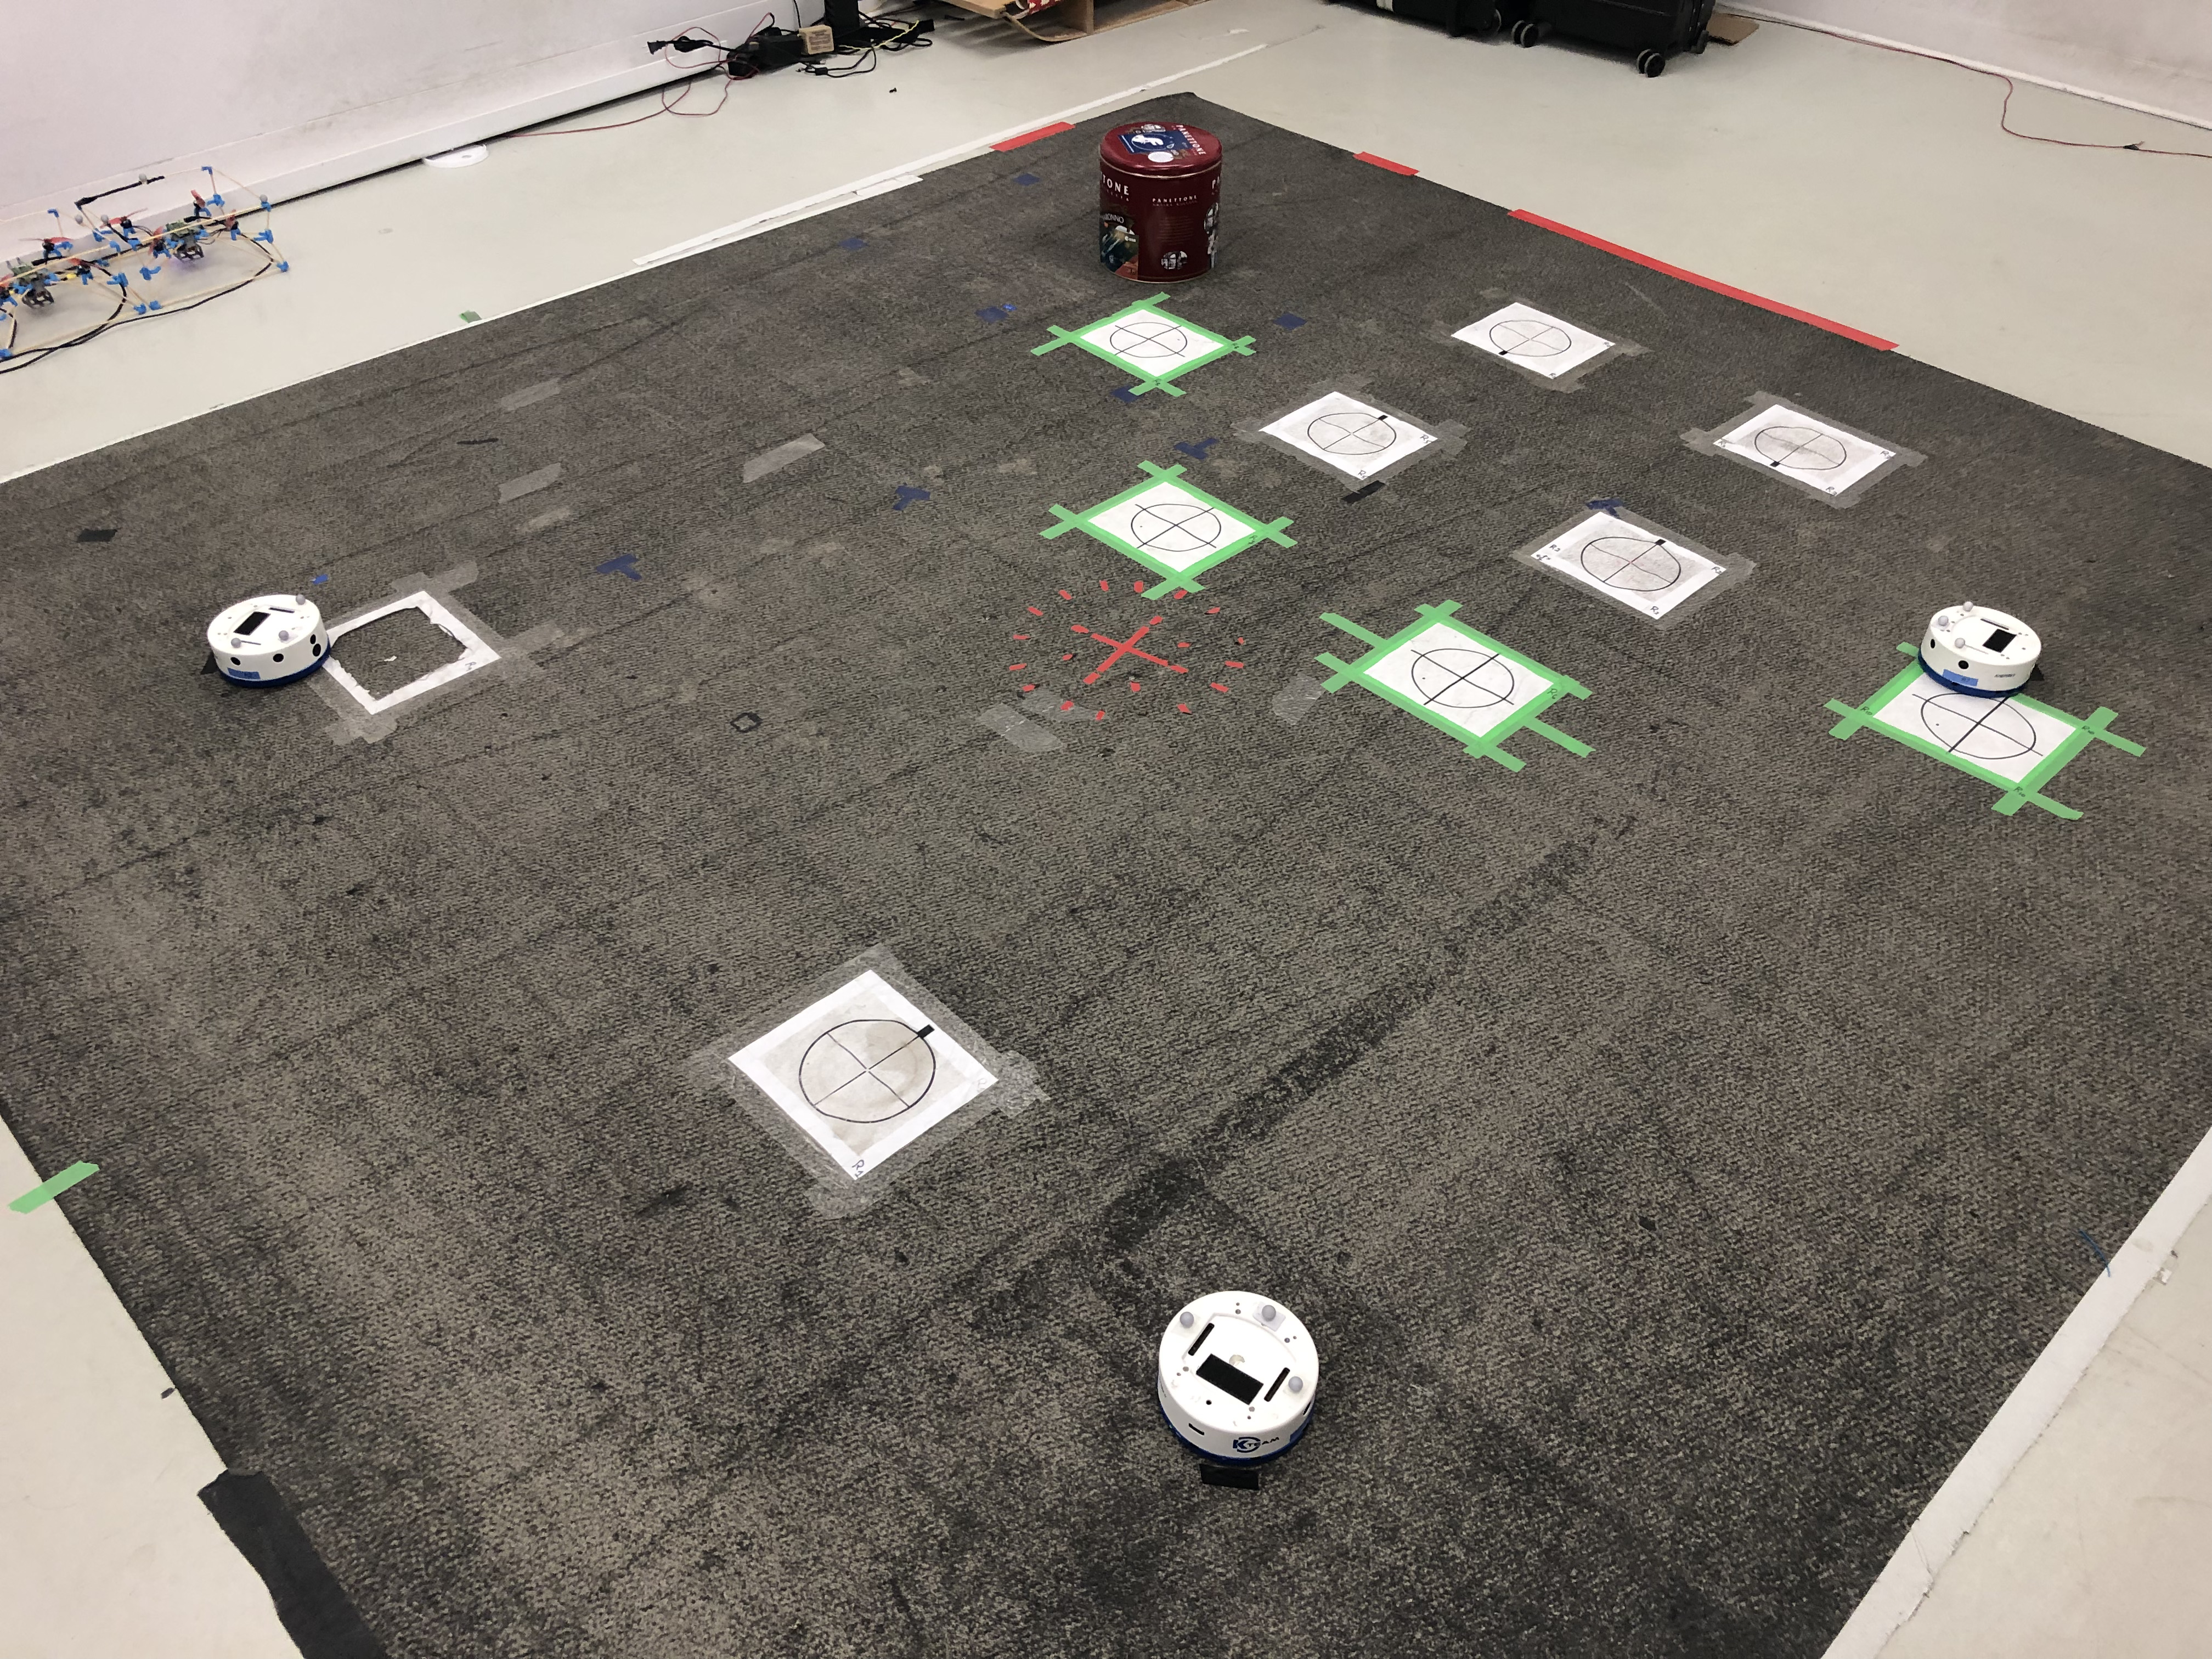
\includegraphics[width=0.99\columnwidth]{images/arena.jpeg}
    \caption{Experiments on three physical KheperaIV robots. The red canister represents the point radiation source in the environment.}
    \label{arena}
\end{figure}